\documentclass[12pt, twoside]{article}
\usepackage[letterpaper, margin=1in, headsep=0.5in]{geometry}
\usepackage[english]{babel}
\usepackage[utf8]{inputenc}
\usepackage{amsmath}
\usepackage{amsfonts}
\usepackage{amssymb}
\usepackage{tikz}
\usetikzlibrary{quotes, angles}
\usepackage{graphicx}
\usepackage{enumitem}
\usepackage{multicol}

\newif\ifmeta
\metatrue %print standards and topics tags

\title{Regents Geometry}
\author{Chris Huson}
\date{September 2020}

\usepackage{fancyhdr}
\pagestyle{fancy}
\fancyhf{}
\renewcommand{\headrulewidth}{0pt} % disable the underline of the header
\raggedbottom


\fancyhead[LE]{\thepage}
\fancyhead[RO]{\thepage \\ Name: \hspace{4cm} \,\\}
\fancyhead[LO]{BECA / Dr. Huson / Geometry 09-Congruence-transformations\\* pset ID: 157}

\begin{document}

\subsubsection*{9-4bCW-Composition}
\begin{enumerate}
\item A transformation is applied to a triangle, $\triangle CAT \rightarrow \triangle C'A'T'$.  Circle True or False to identify each transformation correctly represented below.  \vspace{0.5cm}
    \begin{multicols}{2}
    \begin{itemize}
      \item[T \quad F \quad] Translated six to the left, down two
      \item[T \quad F \quad] Reflected across the $y$-axis
      \item[T \quad F \quad] $(x,y) \rightarrow (x-6, y-2)$
      \item[T \quad F \quad] Reflected across the $y$-axis, then left 2, down 2
      \item[T \quad F \quad] Reflect across $x=-1$
    \end{itemize}
    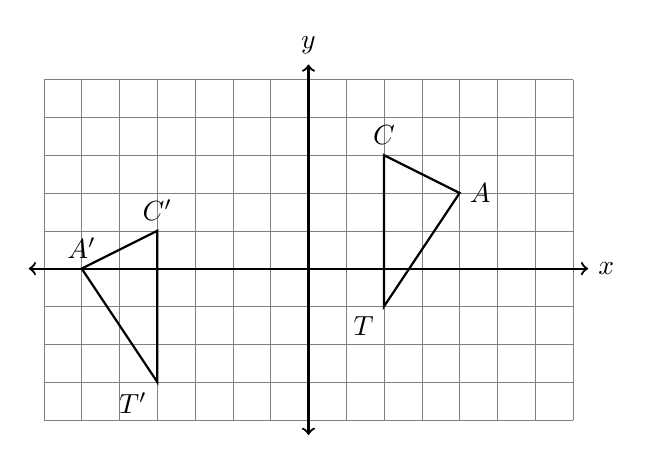
\begin{tikzpicture}[scale=.48]
      \draw [help lines] (-7,-4) grid (7,5);
      \draw [thick, <->] (-7.4,0) -- (7.4,0) node [right] {$x$};
      \draw [thick, <->] (0,-4.4)--(0,5.4) node [above] {$y$};  
      \draw [thick]
      (2,3) node[above] {$C$}--
      (4,2) node[right] {$A$}--
      (2,-1) node[below left] {$T$}--cycle;
      \draw [thick]
      (-4,1) node[above] {$C'$}--
      (-6,0) node[above] {$A'$}--
      (-4,-3) node[below left] {$T'$}--cycle;
    \end{tikzpicture}
  \end{multicols}

\item Determine and state the transformation mapping $\triangle DEF$ onto $\triangle ABC$. Also, make a mapping table of the coordinate pairs.
  \begin{flushright}
      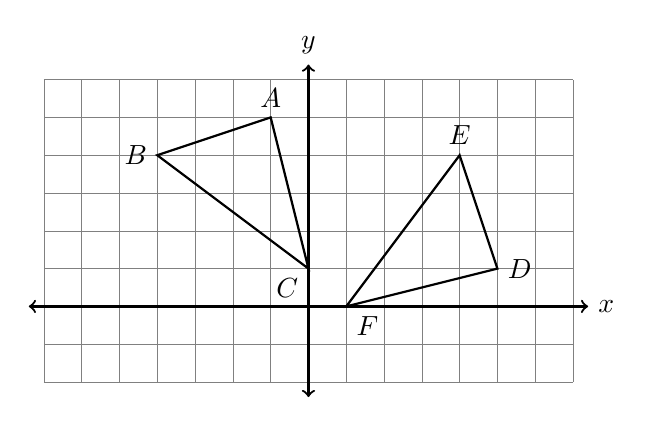
\begin{tikzpicture}[scale=.48]
      \draw [help lines] (-7,-2) grid (7,6);
      \draw [thick, <->] (-7.4,0) -- (7.4,0) node [right] {$x$};
      \draw [thick, <->] (0,-2.4)--(0,6.4) node [above] {$y$};  
      \draw [thick]
        (-1,5) node[above] {$A$}--
        (-4,4) node[left] {$B$}--
        (0,1) node[below left] {$C$}--cycle;
      \draw [thick]
      (5,1) node[right] {$D$}--
      (4,4) node[above] {$E$}--
      (1,0) node[below right] {$F$}--cycle;
    \end{tikzpicture}
  \end{flushright}

\item First reflect the trapezoid $BECA$ across the $y$-axis, then move it down five and right two. Label the images $B'E'C'A'$ and $B''E''C''A''$.
  \begin{center}
      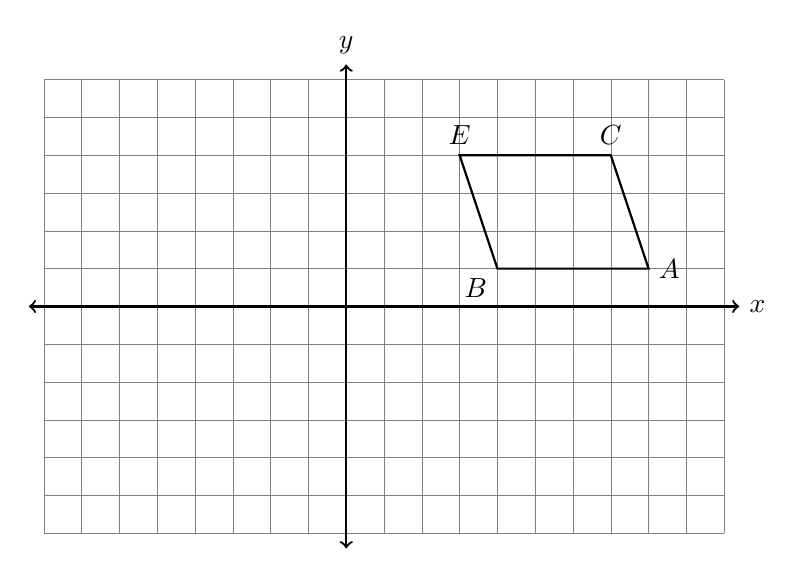
\begin{tikzpicture}[scale=.48]
      \draw [help lines] (-8,-6) grid (10,6);
      \draw [thick, <->] (-8.4,0) -- (10.4,0) node [right] {$x$};
      \draw [thick, <->] (0,-6.4)--(0,6.4) node [above] {$y$};  
      \draw [thick]
        (4,1) node[below left] {$B$}--
        (3,4) node[above] {$E$}--
        (7,4) node[above] {$C$}--
        (8,1) node[right] {$A$}--cycle;  
    \end{tikzpicture}
  \end{center}

\newpage
\item Two transformations have been applied to a triangle in the diagram below, \\$\triangle ABC \rightarrow \triangle A'B'C' \rightarrow \triangle A''B''C''$. Fully characterize each transformation.
    \begin{flushright}
        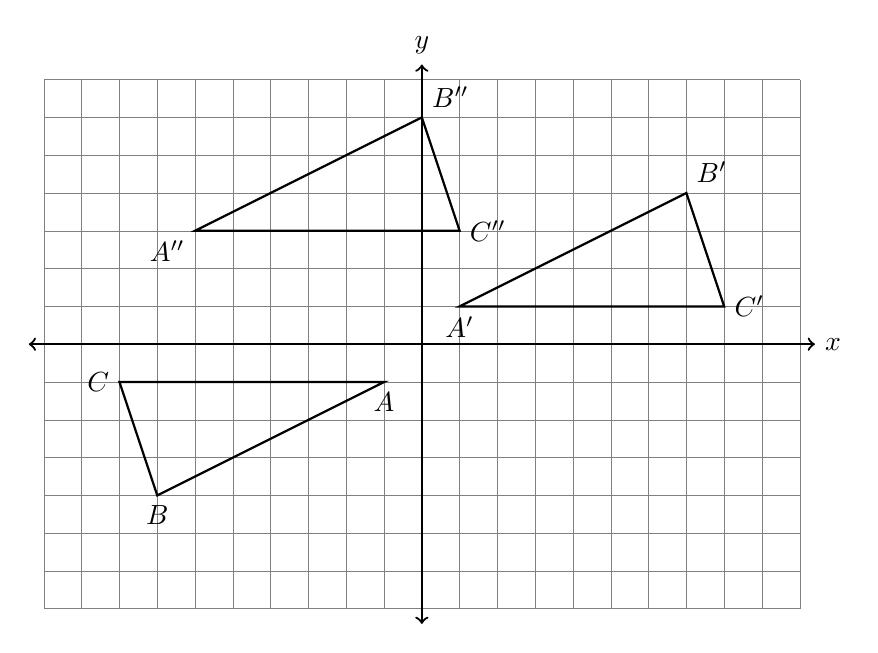
\begin{tikzpicture}[scale=.48]
        \draw [help lines] (-10,-7) grid (10,7);
        \draw [thick, <->] (-10.4,0) -- (10.4,0) node [right] {$x$};
        \draw [thick, <->] (0,-7.4)--(0,7.4) node [above] {$y$};  
        \draw [thick]
          (-6,3) node[below left] {$A''$}--
          (0,6) node[above right] {$B''$}--
          (1,3) node[right] {$C''$}--cycle;
        \draw [thick]
          (1,1) node[below] {$A'$}--
          (7,4) node[above right] {$B'$}--
          (8,1) node[right] {$C'$}--cycle;  
          \draw [thick]
          (-1,-1) node[below] {$A$}--
          (-7,-4) node[below] {$B$}--
          (-8,-1) node[left] {$C$}--cycle;
      \end{tikzpicture}
    \end{flushright} \vspace{2cm}

\item The quadrilateral $ROCK$ undergoes two transformations, shown below. Describe the sequence of transformations applied.
  \begin{flushright}
      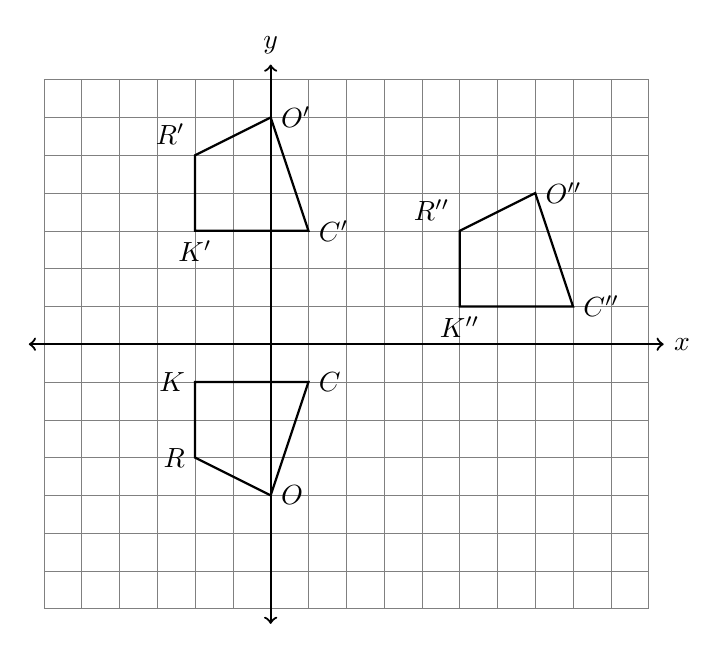
\begin{tikzpicture}[scale=.48]
      \draw [help lines] (-6,-7) grid (10,7);
      \draw [thick, <->] (-6.4,0) -- (10.4,0) node [right] {$x$};
      \draw [thick, <->] (0,-7.4)--(0,7.4) node [above] {$y$};  
      \draw [thick]
        (5,1) node[below] {$K''$}--
        (5,3) node[above left] {$R''$}--
        (7,4) node[right] {$O''$}--
        (8,1) node[right] {$C''$}--cycle;
      \draw [thick]
        (-2,3) node[below] {$K'$}--
        (-2,5) node[above left] {$R'$}--
        (0,6) node[right] {$O'$}--
        (1,3) node[right] {$C'$}--cycle;  
      \draw [thick]
      (-2,-1) node[left] {$K$}--
      (-2,-3) node[left] {$R$}--
      (0,-4) node[right] {$O$}--
      (1,-1) node[right] {$C$}--cycle;
    \end{tikzpicture}
  \end{flushright}


\end{enumerate}
\end{document}